\newpage
\section{Polarization}
Recall the general solution of electromagnectic waves progating in the z-direction. The oscillating electric field components are generally given by
\begin{align*}
    \vec{E}: \, E_x(z,t)=&E_{0x}\cos(kz-\omega t+\phi_x)\\
    E_y(z,t)=&E_{0y}\cos(kz-\omega t+\phi_y)\\
    E_z=&0
\end{align*}

\subsection{Polarization and Mathematical Description}
\subsubsection{Polarization}
Light is a transverse electromagnectic wave. Tus far we have considered only light for which the orientation of the electric field is constant, although its magnitude and sign vary in time. In general, we can condiser two such harmonic lightwaves of the same frequency, moving through the same region of space, in the same direction $\hat{z}$
\begin{align*}
    \vec{E}_x(z,t)=&\hat{i}E_{0x}\cos(kz-\omega t)\\
    \vec{E}_y(z,t)=&\hat{j}E_{0y}\cos(kz-\omega t+ \epsilon)
\end{align*}

\highlight{Linear polarization}: If $epsilon$ is zero or an integral multiple of $\pm 2\pi$, the resultant wave is
\begin{align*}
    \vec{E}=&\vec{E}_x+\vec{E}_y\\
    =&\left(\hat{i}E_{0x}+\hat{j}E_{0y}\right)\cos(kz-\omega t)
\end{align*}

\begin{figure}[H]
    \centering
    \includegraphics[width=0.479\textwidth]{Lec20/Linear polarization}
    \caption{Linear polarization}
\end{figure}

\highlight{Circular polarization}: 
\begin{figure}[H]
    \centering
    \includegraphics[width=0.309\textwidth]{Lec20/Circular polarization}
    \caption{Circular polarization}
\end{figure}
\begin{enumerate}
    \item When both constituent waves have equal amplitudes $(E_{0x}=E_{0y}=E_{0})$ and their relative phase difference $\epsilon=-\frac{\pi}{2}+2m\pi$, where $m$ is an integer, the resultant wave is
    \begin{align*}
        \vec{E}=&\hat{i}E_0\cos(kz-\omega t)+\hat{j}E_0\cos(kz-\omega t-\frac{\pi}{2})\\
        =&E_0\left[ \hat{i}\cos(kz-\omega t)+\hat{j}\sin(kz-\omega t) \right]
    \end{align*}
    
    The resultant $\vec{E}$ is rotating clockwise at an angular frequency of  $\omega$, as seen by an observer toward whom the light is moving. This is referred to as \highlight{right-circular polarized}. The $\vec{E}$-vector makes one complete rotation as the wave advances through one wavelength. 
    \item When their relative phase difference $\epsilon=\frac{\pi}{2}+2m\pi$, where $m$ is an integer, the resultant wave is 
    \begin{align*}
        \vec{E}=&\hat{i}E_0\cos(kz-\omega t)+\hat{j}E_0\cos(kz-\omega t+\frac{\pi}{2})\\
        =&E_0\left[ \hat{i}\cos(kz-\omega t)-\hat{j}\sin(kz-\omega t) \right]
    \end{align*}
    The amplitudes is unaffected, but $\vec{E}$ now rotates counterclockwise, and the wave is \highlight{left-circular polarized}. 
\end{enumerate}

A linearly polarized wave can be synthesized from two oppositely polarized circular waves of equal amplitude. 

\subsubsection{A Math Description of Polarization}
Written in column and complex form, this Jones vector is 
\begin{align*}
    \vec{E}=&\begin{bmatrix}
        E_x(t)\\E_y(t)
    \end{bmatrix}\\
    =&\begin{bmatrix}
        E_{0x}e^{i(kz-\omega t+\phi_x)}\\
        E_{0y}e^{i(kz-\omega t+\phi_y)}
    \end{bmatrix}
\end{align*}

In many applications it is not necessary to know the exact amplitudes and phases. We can rewrite the Jones vector by
\begin{align*}
    \tilde{E}=\begin{bmatrix}
        E_{0x}e^{i\phi_x}\\E_{0y}e^{i\phi_y}
    \end{bmatrix}
\end{align*}

Horizontal and vertical linearly polarized are thus given by
\begin{align*}
    \ket{H}=&\begin{pmatrix}
        1\\0
    \end{pmatrix}\\
    \ket{V}=&\begin{pmatrix}
        0\\1
    \end{pmatrix}
\end{align*}
\begin{figure}[H]
    \centering
    \begin{tikzpicture}
        \draw [<->] (-1.5,0)--(-0.5,0);
        \node at (-1,-1) {$\ket{H}$};
        \draw [<->] (1,0.5)--(1,-0.5); 
        \node at (1,-1) {$\ket{V}$};
    \end{tikzpicture}
    \caption{Horizontal and vertical linearly polarized}
\end{figure}

Linearly polarized at $+ 45 at^{\circ}$ from the x-axis (diagonal) and at $- 45 at^{\circ}$ from the x-axis (anti-diagonal) are given by
\begin{align*}
    \ket{D}=&\frac{1}{\sqrt{2}}\left(\ket{H}+\ket{V}\right)\\
    =&\frac{1}{\sqrt{2}}\begin{pmatrix}
        1\\1
    \end{pmatrix}\\
    \ket{A}=&\frac{1}{\sqrt{2}}\left(\ket{H}-\ket{V}\right)\\
    =&\frac{1}{\sqrt{2}}\begin{pmatrix}
        1\\-1
    \end{pmatrix}
\end{align*}
\begin{figure}[H]
    \centering
    \begin{tikzpicture}
        \draw [<->] (-1.5,-0.5)--(-0.5,0.5);
        \node at (-1,-1) {$\ket{D}$};
        \draw [<->] (0.5,0.5)--(1.5,-0.5); 
        \node at (1,-1) {$\ket{A}$};
    \end{tikzpicture}
    \caption{Diagonal and anti-diagonal linearly polarized}
\end{figure}
Note that we are only interested in polarization, so the vectors are normalized, or in one unit length. 

Right-circular light and left-circular light is given by
\begin{align*}
    \ket{R}=&\frac{1}{\sqrt{2}}\left( \ket{H}-i\ket{V} \right)\\
    =&\frac{1}{\sqrt{2}}\begin{pmatrix}
        1\\-i
    \end{pmatrix}\\
    \ket{L}=&\frac{1}{\sqrt{2}}\left( \ket{H}+i\ket{V} \right)\\
    =&\frac{1}{\sqrt{2}}\begin{pmatrix}
        1\\i
    \end{pmatrix}
\end{align*}
\begin{figure}[H]
    \centering
    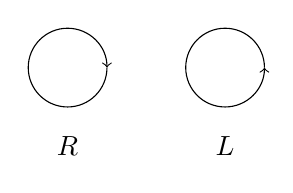
\begin{tikzpicture}
        \draw [<-] (-0.5,0) arc (0:360:0.5);
        \node at (-1,-1) {$\ket{R}$};
        \draw [->] (1.5,0) arc (0:360:0.5);
        \node at (1,-1) {$\ket{L}$};
    \end{tikzpicture}
    \caption{Right-circular light and left-circular light}
\end{figure}

Note that on interference, we discussed the addition in a two-dimensional real space $\mathbb{R}^2$. The space is also equivalent to a one-dimensional complex space $\mathbb{C}^1$, or a two-component real vector space. Now with polarization, we have generalized the one-dimensional complex space $\mathbb{C}^1$ to a two-dimensional complex space $\mathbb{C}^2=\mathbb{C}^1\otimes \mathbb{C}^1$, or a two-component complex vector space (in Jones' vector representation). The additional $\mathbb{C}^1$ space is spanned by the two orthogonal (正交), linearly polarized states $\ket{H}$ and $\ket{V}$. 

Two vectors $\vec{A}$ and $\vec{B}$ are said to be orthogonal when $\vec{A}\cdot\vec{B}=0$, similarly two complex vectors $\vec{A}$ and $\vec{B}$ are said to b orthogonal when $\bra{A} \ket{B} \equiv \tilde{A}^{\dagger }\cdot \tilde{B}=0$. Note that 
\begin{align*}
    \ket{A}=&\tilde{A}\\
    \bra{A}=&\tilde{A}^{\dagger}
\end{align*}
${}^{\dagger}$ means transposed complex conjugation (转置复共轭). 

Any polarization state will have a corresponding orthogonal state. Notice that
\begin{align*}
    \bra{H}\ket{V}=\bra{D}\ket{A}=\bra{L}\ket{R}=0
\end{align*}
As we have seen, any polarization state can be described by a linear combination of the vectors in either one of the orthogonal sets. These same ideas are of considerable importance in quantum mechanics, where deals with orthogonal wave functions. 

\subsection{Monochromatic Light and Natural Light}

\subsubsection{Monochromatic Light}
An idealized \highlight{monochromatic plane wave} must be depicted as an infinite wavetrain. If this disturbance is resolved into two orthogonal components perpendicular to the direction of propagation, they, in turn, must have the same frequency, be infinite in extentm, and therefore be mutually coherent (i.e. $\epsilon=constant$)
\begin{align*}
    \vec{E}_x(z,t)=&\hat{i}E_{0x}\cos(kz-\omega t)\\
    \vec{E}_y(z,t)=&\hat{j}E_{0y}\cos(kz-\omega t+\epsilon)
\end{align*}
\highlight{A perfectly monochromatic plane wave is always polarized. }

The most spectacular of all present-day sources is the laser. Under optimum conditions, with temperature variations and vibrations meticulously suppressed, a laser was actually operated at quite close to its theoretical limit of frequency constancy. 

\subsubsection{Natural Light}
\highlight{Natural light} is composed of a rapidly varying succession $(\sim 10^{-8}s)$ of the different polarization states. It is also known as \highlight{unpolarized} or \highlight{randomly polarized} light. We can mathematical represent natural light in terms of \highlight{two arbitrary, incoherent, orthogonal, linearly polarized waves of equal amplitude} (i.e. waves for which the relative phase difference varies rapidly and randomly). 

Coherence (相干) is a measure of the correlation bewteen the phases measured at different (temporal and spatial) points on a wave. 
\begin{enumerate}
    \item \highlight{Temporal coherence} is a measure of the correlation of light wave's phase at different points \highlight{along the direction of propagation} --- it tells us how monochromatic a source is. 
    \item \highlight{Spatial coherence} is a measure of the correlation of light wave's phase at different points \highlight{transverse to the direction of propagation} --- it tells us how uniform the phase of the wavefront is. 
\end{enumerate}

\begin{figure}[H]
    \centering
    \includegraphics[width=0.309\textwidth]{Lec20/prepare a monochromatic wave that is coherent}
    \caption{how to prepare a monochromatic wave that is both \highlight{ temporally} and \highlight{spatially coherent} from incoherent natural light}
\end{figure}

In reality, light is generally neither completely polarized nor completely unpolarized. More often, the electric-field vector varies in a way that is neither totally regular nor totally irregular, and such an optical disturbance is \highlight{partially polarized}. One useful way of describing this behavior is to envision it as the result of the \highlight{superposition of specific amounts of natural and polarized light}. 

\subsection{Polarizing Sheets}
unpolarized visible light can be transformed into polarized light by sending it through a polarizing sheet, or a polaroid sheet. A polarizing sheet consists of certain long molecules embedded in plastic. When light is then sent through the sheet, \highlight{the electric field component parallel to the polarizing direction is passed (transmitted); the component perpendicular to it is absorbed. }

\begin{figure}[H]
    \centering
    \begin{minipage}{0.22\textwidth}
        \centering
        \includegraphics[width=\textwidth]{Lec20/Polarizing Sheets}
        \caption{\tiny Polarizing Sheets}
    \end{minipage}
    \begin{minipage}{0.18\textwidth}
        \centering
        \includegraphics[width=\textwidth]{Lec20/Polarizing Sheets 1}
        \caption{\small The polarized light emerging from a polarizing sheet}
    \end{minipage}
\end{figure}

Electric field oscillations of \highlight{unpolarized light} can resolve into two components with equal intensity. Therefore, the intensity $I$ of the polarized light emerging from a polarizing sheet is then half the intensity $I_0$ of the original light, i.e.
\begin{align*}
    I=\frac{I_0}{2}
\end{align*}

For \highlight{polarized light}, only the component parallel to the polarizing direction of the sheet $(E_y=E\cos\theta)$ can be transmitted. Therefore, the intensity of the emerging wave is 
\begin{align*}
    I=I_0\cos^2\theta
\end{align*}

If the polarizing directions are parallel, all the light can pass the sheet. If the polarizing directions are perpendicular, no light can pass the sheet. 

\subsection{Polarization by Reflection}
One of the most common sources of polarized light is the ubiquitous process of reflection from dielectric media. Consider a ray of unpolarized light incident on a glass surface. The field $\vec{E}$ of the incident light can be decomposed into two components of equal magnitude, one perpendicular and another parallel to the plane of incidence. In general, the reflected light is \highlight{partially polarized}. 

\begin{figure}[H]
    \centering
    \includegraphics[width=0.309\textwidth]{Lec20/Polarization by Reflection}
    \caption{Polarization by Reflection}
\end{figure}

When the light is incident at a particular incident angle, caleld the \highlight{Brewster angle $\theta_B$}, the reflected light is fully polarized. One finds experimentally that at the incident angle $\theta_B$ the reflected and refracted rays are perpendicular to each other:
\begin{align*}
    \theta_B+\theta_r=90^{\circ}
\end{align*}

According to Snell's law
\begin{align*}
    n_i\sin\theta_B=&n_r\sin\theta_r\\
    =&n_r\sin(90^{\circ}-\theta_B)\\
    =&n_r\cos\theta_B
\end{align*}
or 
\begin{align*}
    \frac{n_r}{n_i}=\tan\theta_B
\end{align*}
If the incident and reflected rays travel in air, we can approximate $n_i$ as unity, so
\begin{align*}
    n_r=\tan\theta_B
\end{align*}